\documentclass[a4paper,12pt]{article}
\usepackage{amssymb}
\usepackage{amsfonts}
\usepackage{amsthm}
\usepackage{amsmath}
\usepackage[T1]{fontenc}
\usepackage[utf8]{inputenc}
\usepackage[british]{babel}
\usepackage{times}
\usepackage{anysize}
\usepackage{color}
\usepackage{listings}
\usepackage{graphicx}
\usepackage{enumerate}
\usepackage{multicol}
\usepackage{float}

\begin{document}
\begin{titlepage}
\center
\vspace*{\fill}
\Huge{Modeling of Physical Systems}\\
\Large{Brownian motion simulation}\\
\vspace*{1.5cm}
Dominik Katszer\\
\large{13 March 2018}
\vspace*{1.5cm}
\vspace*{\fill}
\end{titlepage}
\section{Aim of laboratory}
The aim of this laboratory is to acquaint with the Brownian motion and its characteristics. The next goal is to get knowledge what specific characteristics mean and how they can be interpreted.
\section{Algorithm}
Brownian motion is the random motion of the particles suspended in the fluid (liquid or gas). Sentence above is very important for understanding problem and algorithm. Time is discretised and represented by steps that have passed.

Particle's position during random movement is calculated as previous position plus random value.
$$
x_n = x_{n-1} +d
$$ 
where $x_n$ and $d$ are matrixes $STEP\times DIM$. 

Brownian motion is stimulated by Monte Carlo method which rely on repetead random sampling. Essentail idea of it is to use randomness to solve problem. Program uses normally distributed random numbers to initialize $d$ matrix. It has been achieved by matlab function \verb!randn!.

Implemented algorithm uses many particles for simulation. At the beginning, position of all these particles is set to point 0. Point 0 is described by $N$ parameters depends on dimension and each is set to 0. In each step equastion presented above is applied for each particle. It means that particles are moved step by step by random vector.
\subsection{Parameters}
\begin{itemize}
\item \verb!STEPS! - number of steps of simulation. It can be interpreted as discretised time.
\item \verb!PARTICLES! - number of particles used in simulation.
\item \verb!DIM! - number of dimmensions (1-3).
\end{itemize}

\section{Trajectories}
\label{trajectory}
\begin{figure}[H]
\caption{2D trajectory simulation of 1 particles}
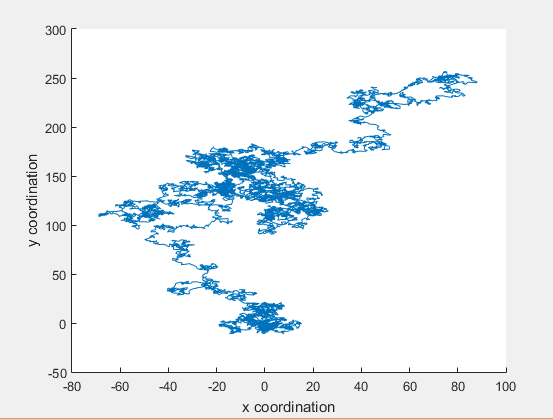
\includegraphics[scale=0.7]{trajectory}
\centering
\end{figure}
\begin{figure}[H]
\caption{2D trajectory simulation of 4 particles}
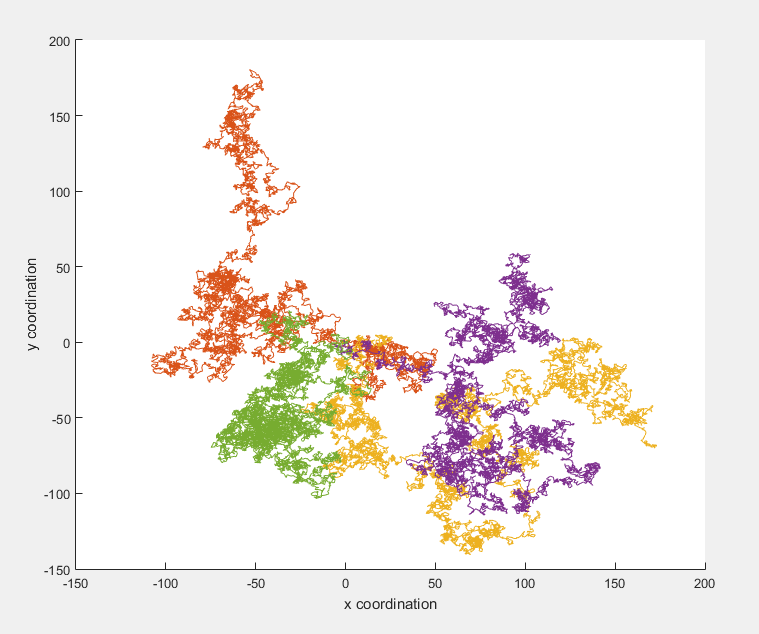
\includegraphics[scale=0.7]{trajectories}
\centering
\end{figure}
\begin{figure}[H]
\caption{3D trajectory simulation of 4 particles}
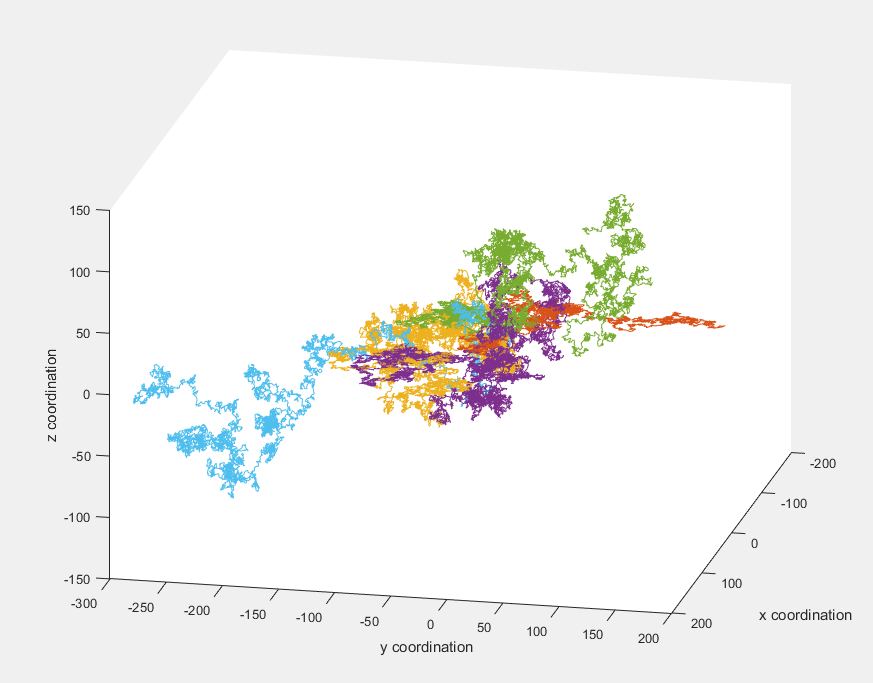
\includegraphics[scale=0.7]{trajectories3d}
\centering
\end{figure}

\section{Self-similarity}
Especially in Figure \ref{trajectory} we can see that result of particle movment tends to group in some places. What is more, values of adjacent steps are similar. Self-similarity is a characteristic which says that object is exactly or approximately similar to a part of itself. 

Comparison of self-similar vector to random genereted vector is presented on the Figure below.

Self-similairity of vector was calculated by comparing this vactor to the same vactor but shifted by $x$ elements.
\begin{figure}[H]
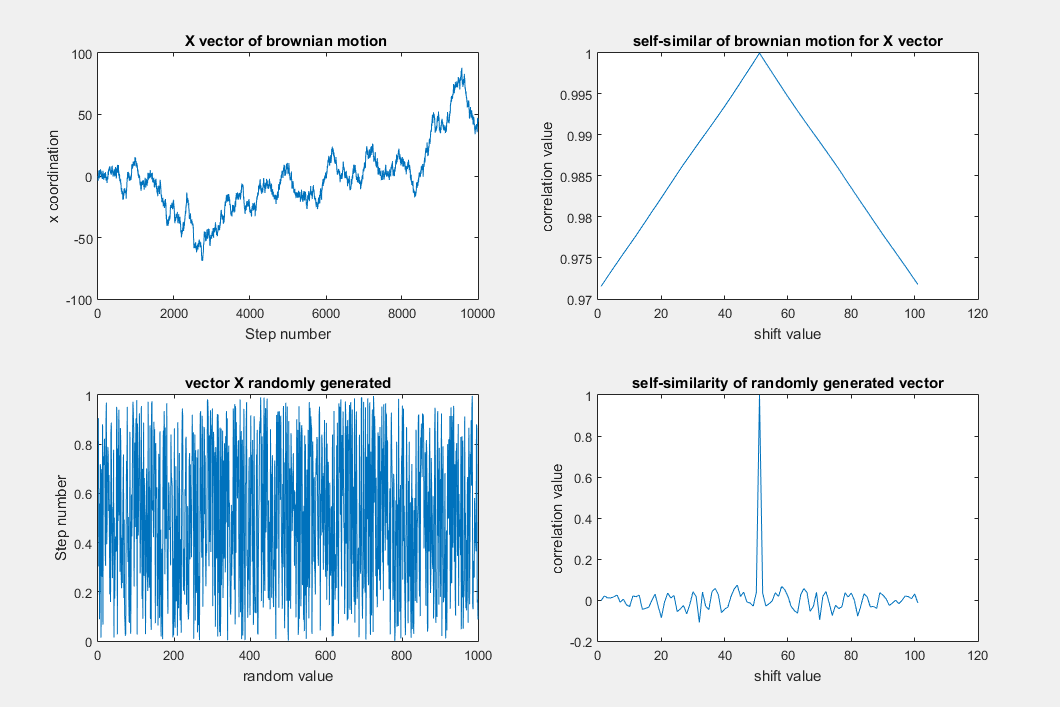
\includegraphics[scale=0.6]{self-similarity}
\centering
\end{figure}

\section{Mean displacement}
In the Figure below we can observe relationship between mean square of displacement and used time  model. Mean was calculated basing on $1000$ particles. It describes the average distance from the center. Additionaly despite of randomness used in algorithm, it shows that in term of mean, particles are moving away the point 0 linearly.
\begin{figure}[H]
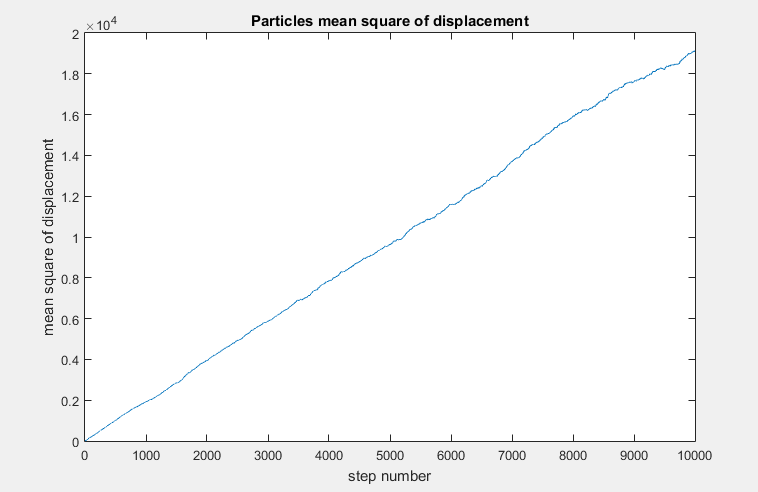
\includegraphics[scale=0.6]{mean-square}
\centering
\end{figure}

\section{Evolution of particles density}
Figures below describe how many particles where in specific state. Taking into considaration figure witch describes 1 dimmension, x values, we can observe that of course the largest value of density is in $x=0$ which is obvoius, because all particles starts from this value. The result represented on figure presents normal distribution. In other words, the greater distance from center is, the smaller density is.
\begin{figure}[H]
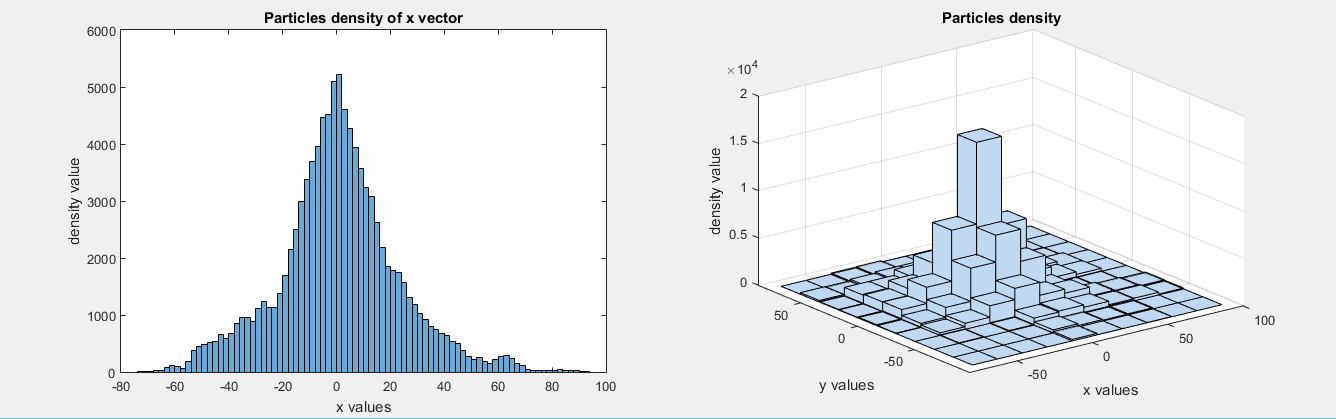
\includegraphics[scale=0.5]{density}
\centering
\end{figure}

\section{Conclusions}
This laboratory has appeared to be a great oportunity to understand a lot of mathematical aspects and brownian motion. What is more, it shows how to anaylize results which often contains a lot of data. After performing simulation we have got knowledge how to interpreate it, and how it is connected with the real world.
\newpage
\section{Source code}
\begin{verbatim}
clear;
clc;

DIM = 2;
PARTICLES = 100;
STEPS = 1000;

displacement = randn(STEPS,DIM,PARTICLES);
trajectory = zeros(STEPS,DIM,PARTICLES);

for i = 2:STEPS
    %Just applying equation for different DIM and PARTICLES
    %It is sum of matrixes, thus we can wrote it one line 
    %for all dims and particles
    trajectory(i,:,:) = trajectory(i-1,:,:) + displacement(i,:,:);
end


%% Just Displaying 
hold on;

for particle = 1:PARTICLES
    if DIM == 1
        plot(trajectory(:,1,particle));
    elseif DIM == 2
        plot(trajectory(:,1,particle), trajectory(:,2,particle));
    elseif DIM == 3
        plot3(
          trajectory(:,1,particle),
          trajectory(:,2,particle),
          trajectory(:,3,particle));
    end    
end
xlabel('x coordination');
ylabel('y coordination');
zlabel('z coordination');
hold off;

%% ONLY FOR TEST 
clc;
test_square = trajectory(2,:,:).^2;
test_sum = sum(test_square,2);
test_mean = mean(test_sum);
%% For good enough results STEPS = 10,000 ; PARTICLES = 1,000

%First element in trajectory is 0,0,0
meanDis = zeros(STEPS,1);
for s = 1:STEPS
    %trajectory(s,:,:).^2  -
        % in each step (rows no), 
        % square all elements (x,y,z) [depends on DIM]
        % do it for all particles
        % -- look at http://matematyka.pisz.pl/strona/1248.html
        % -- in order to understand what is happening
    %sum(A,2) - sum along rows, not colums .
        % 2 descibes dim along with elements will be sumarized 
        % trajectory is 3d (Steps, DIM[x,y,z], PARTICLES)
    %sum(trajectory(s,:,:).^2,2);
        % result of it is square distance from center 
        % for PARTICLE in specific STEP
    %mean(sum(trajectory(s,:,:).^2,2));
        % mean along first dim not 1
        % step is 1 (specified)
        % DIM is 1 - rsult of sum function
        % PARTICLES is not 1
        % it will calculate mean distance from center 
        %for all dims and
    meanDis(s) = mean(sum(trajectory(s,:,:).^2,2));
end
plot(meanDis);
title('Particles mean square of displacement');
xlabel('step number');
ylabel('mean square of displacement');


%% Self Simalirity

Vx = trajectory(:,1,1);
result = [];
SHIFT = 50;
DOUBLE_SHIFT = 2 * SHIFT;
% We compare 2 vectors, element by element.
% If there is no shift then there will be always 1 as result
% because values would be the same.
% If shift is greater then difference is also greater 
%so correlation value is going down
for j = -SHIFT:SHIFT
    %Vx(100:900)  - window to compare
    %Vx(100+j:900+j) - x vector shifted 
    result = [result corr(
       Vx(DOUBLE_SHIFT:STEPS-DOUBLE_SHIFT),
       Vx(DOUBLE_SHIFT+j:STEPS-DOUBLE_SHIFT+j)
      )];
end

subplot(2,2,1);
plot(Vx);
title('X vector of brownian motion ');
xlabel('Step number');
ylabel('x coordination');

subplot(2,2,2);
plot(result);
title('self-similar of brownian motion for X vector');
xlabel('shift value');
ylabel('correlation value');

randomResult=[];
randomX=rand(1000,1);
for i = -50:50
    randomResult = [randomResult corr(
      randomX(100:900),
      randomX(100+i:900+i)
    )];
end
subplot(2,2,3);
plot(randomX);
title('vector X randomly generated');
xlabel('random value');
ylabel('Step number');

subplot(2,2,4);
plot(randomResult);
title('self-similarity of randomly generated vector');
xlabel('shift value');
ylabel('correlation value');

%% Density, good results for STEPS = 1,000 ; PARTICLES = 100

% histogram automatically create bins and count occurence
% in specific range
% X - bins with automatically selected range, steps
% Y - number of particles in specific bin
% in other words
    % It shows that at the begging all particles 
    % starts from the same x,
    % after few steps they are slowly move away from each other
    %and finally each particle is in differnet bin.
xAllParticles = trajectory(:,1,:);
yAllParticles = trajectory(:,2,:);
figure(1);
histogram(xAllParticles);
title('Particles density of x vector');
xlabel('step');
ylabel('density value');

%figure(2);
%histogram(yAllParticles);


allX = reshape(xAllParticles, [STEPS*PARTICLES,1] );
allY = reshape(yAllParticles, [STEPS*PARTICLES,1] );
figure(3);
hist3([allX, allY])
title('Particles density');
xlabel('x');
ylabel('y');
zlabel('density value');


%% ONLY FOR TEST hist3

% we provide x and y (floor) and z axis will described density
load seamount;
dat = [-y,x];
hist3(dat);
\end{verbatim}
\end{document}